%\documentclass[fleqn]{book}
\documentclass[11pt]{amsbook}

\usepackage[turkish]{babel}

%\usepackage{../HBSuerDemir}	% ------------------------
\usepackage{../Ceyhun}	% ------------------------
\usepackage{../amsTurkish}


\begin{document}
% ++++++++++++++++++++++++++++++++++++++
\hPage{174}
% ++++++++++++++++++++++++++++++++++++++


\begin{figure}[htb]
	\centering
	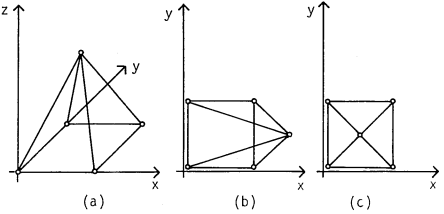
\includegraphics[width=1\textwidth]{images/figure1.png}
	
\end{figure}


\begin{figurename}
    4.1.1 Ç(5,8) çizgesinin değisik çizimleri.
düğümlerde kesisen bir çizimle sonuçlanabilir. Bu
gözlemin sonucu olarak, 'Her çizge, ayrıtları
yalnız düğümlerde kesisecek biçimde düzleme
çizilebilir mi ?' gibi bir soru aklımıza gelebilir. 
Şekil 4.1 .2 de gösterilen İ(4,3) çizgesini
incelersek, böyle bir sorunun karşılığını, 'her
    
\end{figurename}
    
    
\begin{figure}[htb]
	\centering
	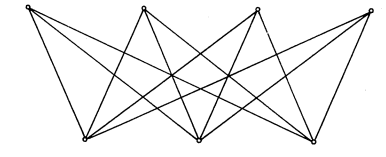
\includegraphics[width=1\textwidth]{images/figure2.png}
	\caption{Şekil 4.1.2 Düzleme çizilemeyen İ(4,3) çizgesi.}
	
\end{figure}
    
\end{document}



